\documentclass[../../../interview-questions.tex]{subfiles}

\begin{document}

\subsection{Java线程池}

\paragraph{Java线程池原理}

J.U.C提供的线程池:ThreadPoolExecutor类,帮助开发人员管理线程并方便地执行并行任务。了解并合理使用线程池,是一个开发人员必修的基本功。线程过多会带来额外的开销,其中包括创建销毁线程的开销、调度线程的开销等等,同时也降低了计算机的整体性能。线程池维护多个线程,等待监督管理者分配可并发执行的任务。这种做法,一方面避免了处理任务时创建销毁线程开销的代价,另一方面避免了线程数量膨胀导致的过分调度问题,保证了对内核的充分利用\footnote{参见:\url{https://tech.meituan.com/2020/04/02/java-pooling-pratice-in-meituan.html}}。JUC是java.util.concurrent包的简称,在Java5.0添加,目的就是为了更好的支持高并发任务。

\paragraph{JVM线程池任务调度(线程池任务添加流程)}

任务调度是线程池的主要入口,当用户提交了一个任务,接下来这个任务将如何执行都是由这个阶段决定的。了解这部分就相当于了解了线程池的核心运行机制。

首先,所有任务的调度都是由execute方法完成的,这部分完成的工作是:检查现在线程池的运行状态、运行线程数、运行策略,决定接下来执行的流程,是直接申请线程执行,或是缓冲到队列中执行,亦或是直接拒绝该任务。其执行过程如下:

首先检测线程池运行状态,如果不是RUNNING,则直接拒绝,线程池要保证在RUNNING的状态下执行任务。
如果workerCount < corePoolSize,则创建并启动一个线程来执行新提交的任务。
如果workerCount >= corePoolSize,且线程池内的阻塞队列未满,则将任务添加到该阻塞队列中。
如果workerCount >= corePoolSize \&\& workerCount < maximumPoolSize,且线程池内的阻塞队列已满,则创建并启动一个线程来执行新提交的任务。
如果workerCount >= maximumPoolSize,并且线程池内的阻塞队列已满, 则根据拒绝策略来处理该任务, 默认的处理方式是直接抛异常。

\paragraph{线程池主要组件}

一个线程池包括以下四个基本组成部分:

\begin{enumerate}
    \item {线程池管理器(ThreadPoolManager):用于创建并管理线程池,包括 创建线程池,销毁线程池,添加新任务;}
    \item {工作线程(WorkThread):线程池中线程,在没有任务时处于等待状态,可以循环的执行任务;}
    \item {任务接口(Task):每个任务必须实现的接口,以供工作线程调度任务的执行,它主要规定了任务的入口,任务执行完后的收尾工作,任务的执行状态等;}
    \item {任务队列(taskQueue):用于存放没有处理的任务。提供一种缓冲机制。}
\end{enumerate}


\paragraph{创建一个线程池需要输入几个参数}

\textbf{corePoolSize(线程池的基本大小)}:当提交一个任务到线程池时,线程池会创建一个线程来执行任务,即使其他空闲的基本线程能够执行新任务也会创建线程,等到需要执行的任务数大于线程池基本大小时就不再创建。如果调用了线程池的prestartAllCoreThreads方法,线程池会提前创建并启动所有基本线程。

\textbf{maximumPoolSize(线程池最大大小)}:线程池允许创建的最大线程数。如果队列满了,并且已创建的线程数小于最大线程数,则线程池会再创建新的线程执行任务。值得注意的是如果使用了无界的任务队列这个参数就没什么效果。

\textbf{runnableTaskQueue(任务队列)}:用于保存等待执行的任务的阻塞队列。有几种队列类型,提交队列、有界任务队列、无界任务队列、优先任务队列。

\begin{enumerate}
    \item {有界队列:SynchronousQueue :一个不存储元素的阻塞队列,每个插入操作必须等到另一个线程调用移除操作,否则插入操作一直处于 阻塞状态,吞吐量通常要高于LinkedBlockingQueue,静态工厂方法 Executors.newCachedThreadPool 使用了这个队列。}
    \item {有界的任务队列:ArrayBlockingQueue:一个由数组支持的有界阻塞队列。此队列按 FIFO(先进先出)原则对元素进行排序。一旦创建了这样的缓存区,就不能再增加其容量。试图向已满队列中放入元素会导致操作受阻塞;试图从空队列中提取元素将导致类似阻塞。}使用ArrayBlockingQueue有界任务队列,若有新的任务需要执行时,线程池会创建新的线程,直到创建的线程数量达到corePoolSize时,则会将新的任务加入到等待队列中。若等待队列已满,即超过ArrayBlockingQueue初始化的容量,则继续创建线程,直到线程数量达到maximumPoolSize设置的最大线程数量,若大于maximumPoolSize则执行拒绝策略。在这种情况下,线程数量的上限与有界任务队列的状态有直接关系。如果有界队列初始容量较大或者没有达到超负荷的状态,线程数将一直维持在corePoolSize以下,反之当任务队列已满时,则会以maximumPoolSize为最大线程数上限。
    \item {无界队列:LinkedBlockingQueue:基于链表结构的无界阻塞队列,它可以指定容量也可以不指定容量(实际上任何无限容量的队列/栈都是有容量的,这个容量就是Integer.MAX\_VALUE)}
    \item {PriorityBlockingQueue:是一个按照优先级进行内部元素排序的无界阻塞队列。队列中的元素必须实现 Comparable 接口,这样才能通过实现compareTo()方法进行排序。优先级最高的元素将始终排在队列的头部;PriorityBlockingQueue 不会保证优先级一样的元素的排序。}除了第一个任务直接创建线程执行外,其他的任务都被放入了优先任务队列,按优先级进行了重新排列执行,且线程池的线程数一直为corePoolSize,也就是只有一个。通过运行的代码我们可以看出PriorityBlockingQueue它其实是一个特殊的无界队列,它其中无论添加了多少个任务,线程池创建的线程数也不会超过corePoolSize的数量,只不过其他队列一般是按照先进先出的规则处理任务,而PriorityBlockingQueue队列可以自定义规则根据任务的优先级顺序先后执行。
\end{enumerate}

注意:keepAliveTime和maximumPoolSize及BlockingQueue的类型均有关系。如果BlockingQueue是无界的,那么永远不会触发maximumPoolSize,自然keepAliveTime也就没有了意义。


\textbf{RejectedExecutionHandler(拒绝策略,饱和策略)}:当队列和线程池都满了,说明线程池处于饱和状态,那么必须采取一种策略处理提交的新任务。这个策略默认情况下是AbortPolicy,表示无法处理新任务时抛出异常。以下是JDK1.5提供的四种策略。

\begin{enumerate}
    \item {ThreadPoolExecutor.AbortPolicy:丢弃任务并抛出RejectedExecutionException异常。}
    \item {ThreadPoolExecutor.DiscardPolicy:也是丢弃任务,但是不抛出异常。}
    \item {ThreadPoolExecutor.DiscardOldestPolicy:丢弃队列最前面的任务,然后重新尝试执行任务(重复此过程)}
    \item {ThreadPoolExecutor.CallerRunsPolicy:由调用线程处理该任务}
\end{enumerate}

\textbf{keepAliveTime(线程活动保持时间,线程池的工作线程空闲后​​​,​​保持存活的时间​​​)}:线程池的工作线程空闲后,保持存活的时间。所以如果任务很多,并且每个任务执行的时间比较短,可以调大这个时间,提高线程的利用率。

\textbf{TimeUnit(线程活动保持时间的单位)}:可选的单位有天(DAYS),小时(HOURS),分钟(MINUTES),毫秒(MILLISECONDS),微秒(MICROSECONDS, 千分之一毫秒)和毫微秒(NANOSECONDS, 千分之一微秒)。

\textbf{ThreadFactory 线程创建工厂}ThreadFactory:用于设置创建线程的工厂,可以通过线程工厂给每个创建出来的线程设置更有意义的名字,Debug和定位问题时非常有帮助。

\paragraph{线程池5个状态}\label{threadpoolcaption}

线程池的5种状态:Running、ShutDown、Stop、Tidying、Terminated。

\textbf{Running}(1) 状态说明:线程池处在RUNNING状态时,能够接收新任务,以及对已添加的任务进行处理。
(2) 状态切换:线程池的初始化状态是RUNNING。换句话说,线程池被一旦被创建,就处于RUNNING状态,并且线程池中的任务数为0!

\begin{figure}[htbp]
	\centering
	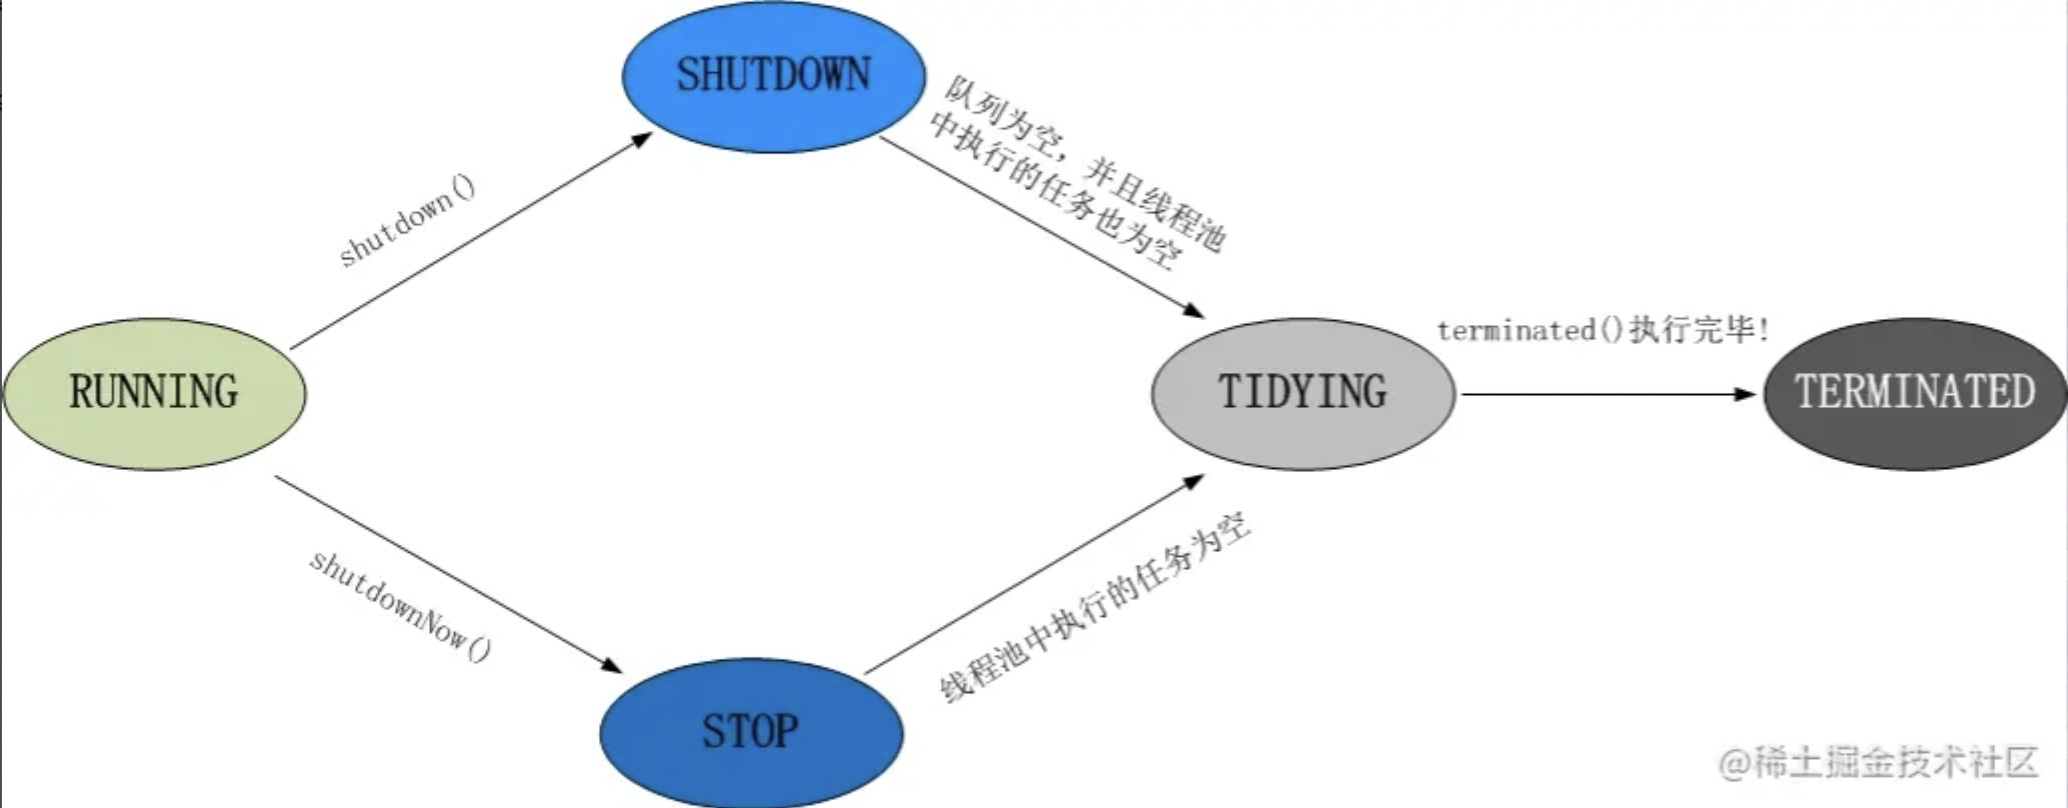
\includegraphics[scale=0.15]{threadpollstatus.jpg}
	\caption{线程池状态}
	\label{fig:threadpollstatus}
\end{figure}

当线程池调用shutDown()方法时,线程池的状态则立刻变成SHUTDOWN状态。此时,则不能再往线程池中添加任何任务,否则将会抛出RejectedExecutionException异常。但是,此时线程池不会立刻退出,直到添加到线程池中的任务都已经处理完成,才会退出。执行shutDownNow()方法,线程池的状态立刻变成STOP状态,并试图停止所有正在执行的线程,不再处理还在池队列中等待的任务,当然,它会返回那些未执行的任务。 
它试图终止线程的方法是通过调用Thread.interrupt()方法来实现的,但是大家知道,这种方法的作用有限,如果线程中没有sleep 、wait、Condition、定时锁等应用, interrupt()方法是无法中断当前的线程的。所以,ShutdownNow()并不代表线程池就一定立即就能退出,它可能必须要等待所有正在执行的任务都执行完成了才能退出。 章节\ref{threadcaption}可以参看线程的6种状态。

\paragraph{线程池如何实现线程复用}

线程池可以把线程和任务进行解耦,线程归线程,任务归任务,摆脱了之前通过 Thread 创建线程时的一个线程必须对应一个任务的限制。在线程池中,同一个线程可以从 BlockingQueue 中不断提取新任务来执行,其核心原理在于线程池对 Thread 进行了封装,并不是每次执行任务都会调用 Thread.start() 来创建新线程,而是让每个线程去执行一个“循环任务”,在这个“循环任务”中,不停地检查是否还有任务等待被执行,如果有则直接去执行这个任务,也就是调用任务的 run 方法,把 run 方法当作和普通方法一样的地位去调用,相当于把每个任务的 run() 方法串联了起来,所以线程数量并不增加。实现线程复用的逻辑在ThreadPoolExecutor类的runWorker方法中。这个 while 循环有个 getTask 方法,getTask 的主要作用是阻塞从队列中拿任务出来,如果队列中有任务,那么就可以拿出来执行,如果队列中没有任务,这个线程会一直阻塞到有任务为止(或者超时阻塞)。

\begin{lstlisting}[language=Java]
final void runWorker(Worker w) {
    Thread wt = Thread.currentThread();
    Runnable task = w.firstTask;
    w.firstTask = null;
    w.unlock(); // allow interrupts
    boolean completedAbruptly = true;
    while (task != null || (task = getTask()) != null) {
    }
}
\end{lstlisting}

使用队列的 poll 或 take 方法从队列中拿数据,根据队列的特性,队列中有任务可以返回,队列中无任务会阻塞。注意任务阻塞是不消耗CPU资源的\footnote{参见:\url{https://stackoverflow.com/questions/5895895/does-java-blocked-threads-take-up-more-cpu-resources}}。

\begin{lstlisting}[language=Java]
Runnable r = timed ?
    workQueue.poll(keepAliveTime, TimeUnit.NANOSECONDS) :
    workQueue.take();
\end{lstlisting}
    

线程池的线程复用就是通过取 Worker 的 firstTask 或者通过 getTask 方法从 workQueue 中不停地取任务,并直接调用 Runnable 的 run 方法来执行任务,这样就保证了每个线程都始终在一个循环中,反复获取任务,然后执行任务,从而实现了线程的复用。


\end{document}